% =====================================================================
%  CHAPTER 2 — LITERATURE SURVEY
% =====================================================================
\clearpage
\chapter{Literature Survey}

This chapter surveys the work on which this project builds and against which
it must be positioned. The survey is organised by the six areas the design
touches rather than chronologically, because the contribution of this work
lies precisely at the intersection of two of them --- durable execution and
embedding-based similarity --- that have so far been studied in isolation.

A note on venues is warranted. In distributed systems, the top conferences
--- VLDB, SOSP, CIDR, NeurIPS and IPDPS --- are fully peer-reviewed and carry
standing equal to or greater than most journals. This is the norm of the
subfield rather than a substitute for journal publication. Except where a
foundational result is explicitly identified as such, every work surveyed
here was published between 2020 and 2026.

\section{Durable Execution and Workflow Correctness}

The idea that a long-running computation should be made resilient by recording
its progress rather than by checkpointing its memory is the foundation of this
project. AMBROSIA~\cite{ambrosia2020} framed the property as \emph{virtual
resiliency}: application code is written as though failures do not occur, and
the runtime obtains resilience by logging the messages that cross the
application boundary and replaying them after a crash. AMBROSIA is the
closest published system to this project in intent, and it is also the
sharpest point of comparison on recovery performance; its reported automatic
failover in approximately 1.8 seconds with no loss is better than what this
project achieves, a point returned to in Section~4.1.6 and reported plainly
rather than omitted.

The DBOS line of work makes a different and complementary argument: that the
right place for this machinery is inside a database. The original DBOS
paper~\cite{dbos2022} proposed moving operating-system-level state into a
DBMS, accepting a measured penalty of roughly forty times the cost of a
conventional system call in exchange for transactional state management and
queryable system state. \emph{DBOS: Three Years Later}~\cite{dbos2025}
reported on the practical consequences after the idea had been built out,
describing a durable execution system constructed directly on PostgreSQL.
That paper is the closest academic precedent for this project's central
engineering decision --- persistence-layer durability with no external
orchestrator --- and its stated limitations are instructive: execution is not
partitioned across machines, and calls to external services must still protect
themselves against repetition.

R3~\cite{r3vldb2023} provides the formal treatment of record-and-replay for
database-backed applications, including the \emph{retroaction} capability of
replaying a recorded execution against modified code. Its central limitation
is directly relevant here: external API calls cannot be replayed unless they
are safe to repeat, which is the same boundary this project confronts in its
crash-window analysis.

Most recently, AC/DC~\cite{acdc2026} addressed consistency and correctness
guarantees for data-oriented workflow systems, and contributed two findings
this project uses. The first is the quantitative observation already cited in
Chapter~1, that error-handling logic dominates application code. The second is
an experimental comparison between locking and compensation-based rollback:
when a single workflow step took one second, their locking approach degraded
to approximately two orders per second with 42\% of orders failing, whereas
the step-by-step compensation approach sustained sixteen orders per second
with no failures. That result is the empirical justification for this
project's decision to implement compensation rather than long-held locks, and
it is referenced again in Section~4.2.9.

Netherite~\cite{netherite2022} addressed the efficient execution of serverless
workflows, and is relevant to this work less for its mechanism than for its
evaluation methodology: it reports scaling as a ratio rather than as an
absolute throughput, which is the correct way to report a scaling result
obtained on hardware that differs from the reader's.

\begin{table}[htbp]
  \centering
  \caption{Research on durable execution and workflow correctness}
  \label{tab:durable}
  \small
  \begin{tabular}{@{}p{0.95in}p{0.72in}p{1.52in}p{1.72in}@{}}
    \toprule
    \textbf{Work} & \textbf{Venue, year} & \textbf{Contribution} &
    \textbf{Stated limitation} \\
    \midrule
    AMBROSIA~\cite{ambrosia2020} & PVLDB 2020 &
      Virtual resiliency by logging messages at the application boundary &
      Requires the application to adopt its programming model throughout \\
    DBOS~\cite{dbos2022} & VLDB 2022 &
      Places operating-system state in a DBMS for transactional management &
      Database calls measured at roughly 40$\times$ the cost of a system call \\
    R3~\cite{r3vldb2023} & PVLDB 2023 &
      Formal record--replay--retroaction for database-backed applications &
      External API calls cannot be replayed unless repeatable \\
    Netherite~\cite{netherite2022} & PVLDB 2022 &
      Efficient serverless workflow execution; ratio-based scaling evaluation &
      Reports scaling ratios without absolute baselines \\
    DBOS 3 Years~\cite{dbos2025} & VLDB Journal 2025 &
      Durable execution built directly on PostgreSQL &
      No partitioning across machines; external calls self-protect \\
    AC/DC~\cite{acdc2026} & CIDR 2026 &
      Correctness guarantees and rollback for workflow systems &
      Locking variant: 42\% failures at 1\,s steps; single machine only \\
    \bottomrule
  \end{tabular}
\end{table}

\section{Sharding and Partition Management}

Partitioning execution across machines is a well-understood problem with one
dominant published reference point. Meta's Shard
Manager~\cite{shardmanager2021} analysed hundreds of internal sharded
applications and generalised them into a single framework managing shards
across approximately a million machines. Two findings matter to this project.

The first is architectural confirmation: Shard Manager also separates the
mapping from application key to shard from the mapping of shard to server,
exactly the two-level indirection adopted in Section~4.1.4, and for the same
reason --- it makes rebalancing an assignment change rather than a data
migration.

The second is a limitation this project deliberately avoids. Shard Manager
depends on ZooKeeper for coordination. At Meta's scale that is unremarkable;
at the scale this project targets, a second distributed system whose only job
is to decide who owns what is a substantial and avoidable cost. The
observation that even a system of that sophistication still requires an
external coordinator is the motivating evidence for this project's
persistence-layer alternative.

\begin{table}[htbp]
  \centering
  \caption{Production workflow orchestrators and the infrastructure each
    requires, from their own deployment documentation}
  \label{tab:orchestrators}
  \small
  \begin{tabular}{@{}p{0.85in}p{0.62in}p{1.52in}p{1.92in}@{}}
    \toprule
    \textbf{System} & \textbf{Origin} & \textbf{Purpose} &
    \textbf{Components required} \\
    \midrule
    Cadence & Uber & Long-running business processes; $\approx$12 billion task
      runs per month & Cassandra or MySQL, queues, timer service, matching
      service, workers \\
    Conductor & Netflix & Video encoding and delivery pipelines running for days
      & Database, Elasticsearch, queues, central server, workers \\
    Airflow & Apache & Scheduled data pipelines &
      PostgreSQL, Redis or RabbitMQ, scheduler, Celery workers \\
    Quartz & Enterprise Java & Scheduled jobs across many servers without
      duplication & Shared database with row locks \\
    Temporal & Temporal & General-purpose durable execution &
      Datastore, history service, matching service, frontend \\
    Restate & Restate & Log-native durable execution &
      Built-in replicated log and embedded RocksDB \\
    \midrule
    \textbf{durexec} & \textbf{This work} & \textbf{General-purpose durable
      execution} & \textbf{PostgreSQL} \\
    \bottomrule
  \end{tabular}
\end{table}

\section{Ownership, Coordination and Fencing}

The question of which machine is allowed to act on behalf of a partition at a
given instant is the hardest correctness problem in a sharded system, because
the failure mode is silent. A node that has been frozen by a
garbage-collection pause or a virtual-machine suspension has no way to detect
that time has passed, and will resume in the sincere belief that it still
holds a lease that has in fact expired and been granted to someone else.

The canonical treatments of this problem are Raft, which obtains agreement
through an explicit consensus protocol at the cost of operating a dedicated
cluster, and the \emph{fencing token} argument, which observes that a lease is
not sufficient and that the protected resource must itself reject writes
carrying a stale token~\cite{kleppmann2017}. Temporal implements precisely
this idea in its persistence layer under the name \emph{RangeID}.

The design adopted in Section~4.1.5 follows the fencing-token argument but
places the check inside the database transaction that performs the write,
using \cd{SELECT \ldots{} FOR UPDATE} to serialise the two. Nothing in this
mechanism is novel in isolation; what is claimed is that the combination is
sufficient, that it removes the need for ZooKeeper in a system of this scale,
and that its cost --- the database becomes the coordination bottleneck and the
availability floor --- is acceptable and should be stated rather than
concealed.

\begin{figure}[htbp]
  \centering
  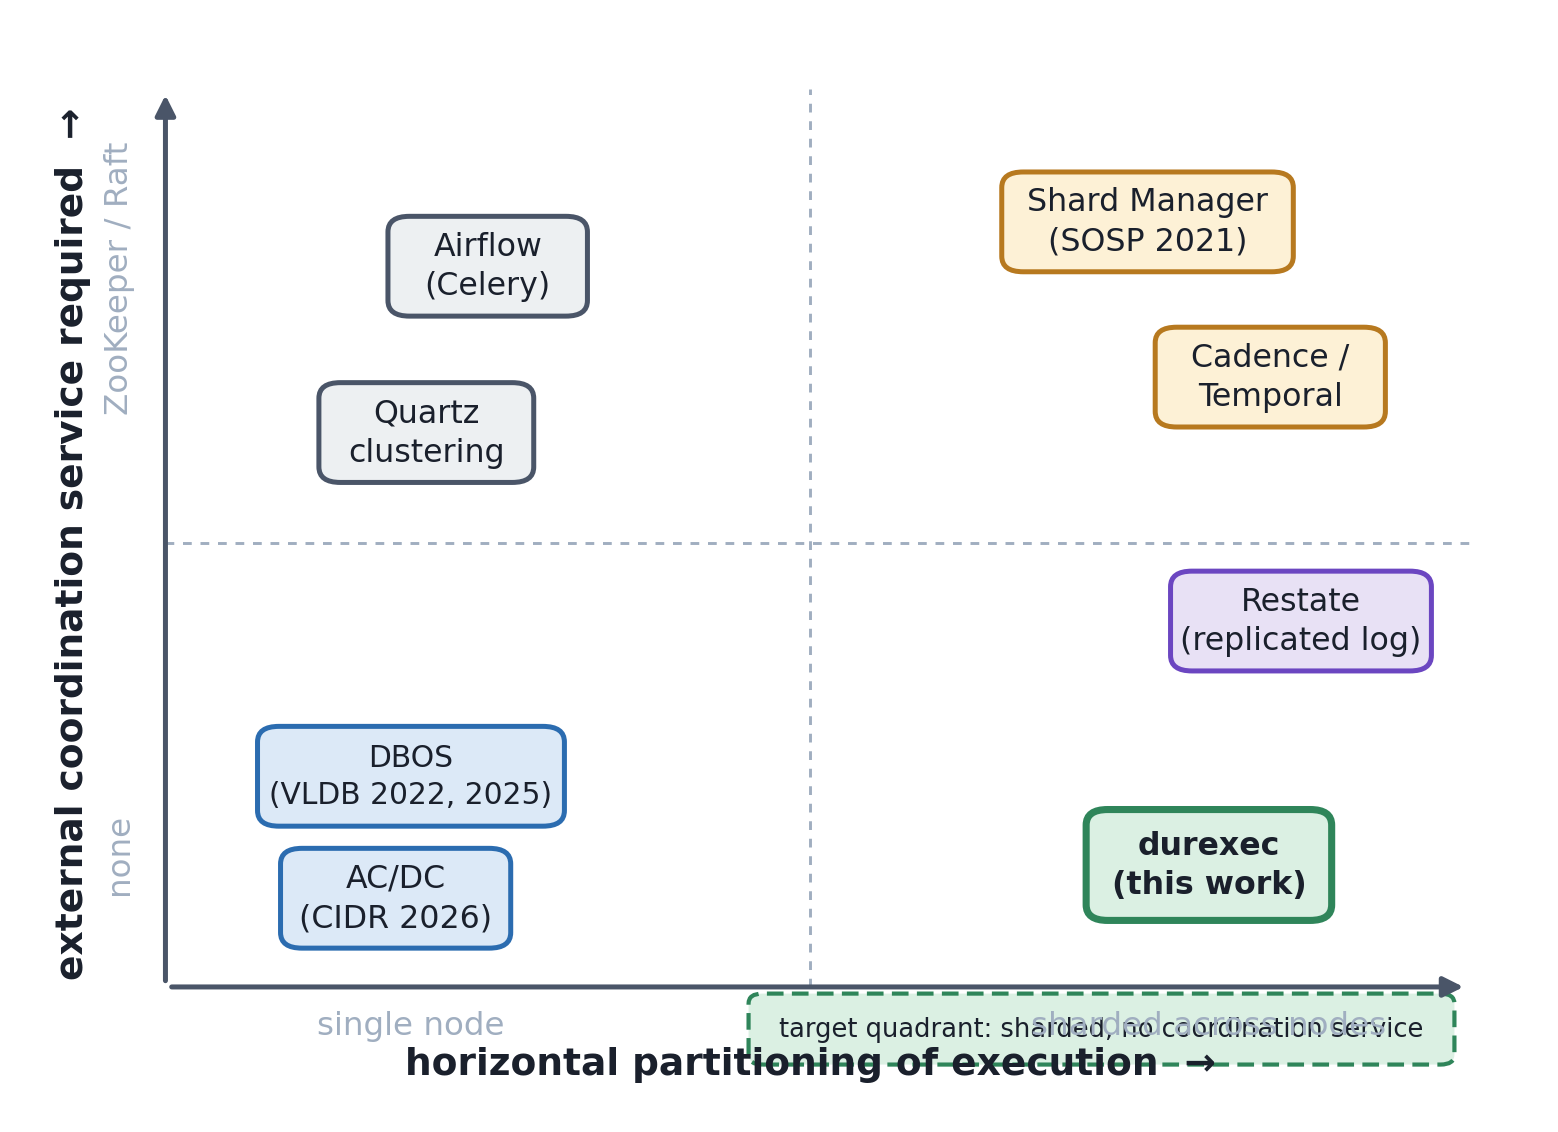
\includegraphics[width=0.94\linewidth]{figures/fig_2_1_related_work_map.png}
  \caption{Positioning of the surveyed systems on the two axes this project
    cares about. Systems in the upper half require a coordination service
    outside their data store; systems in the right half partition execution
    across machines. The lower-right quadrant --- partitioned without a
    coordination service --- is the target of this work.}
  \label{fig:relatedmap}
\end{figure}

\section{The Saga Pattern and Compensation}

When a multi-step transaction fails partway through and its completed steps
cannot be rolled back by the database, the established remedy is the saga: run
a compensating action for each completed step, in reverse order. The pattern
originates in Garcia-Molina and Salem's 1987 formulation~\cite{sagas1987},
included here as the foundational reference despite falling outside the
recency window of this survey.

Recent work has extended it in two directions relevant to this project.
Daraghmi et al.~\cite{daraghmi2022} addressed the saga's lack of isolation ---
the fact that other transactions can observe intermediate states between a
step and its compensation --- by introducing a quota cache. This project does
not solve that problem, and Section~4.2.9 states plainly that it accepts the
limitation rather than addressing it. Reza and Rahman~\cite{reza2023} provide
a formal extension of saga and microservice patterns for resilient distributed
transactions.

The most directly competing work is Robust Agent Compensation
(RAC)~\cite{rac2026}, a log-based compensation framework built specifically
for AI agents, which uses the Model Context Protocol to discover compensation
pairs. RAC and this project address adjacent halves of the same problem and
the distinction is worth stating precisely: \textbf{RAC undoes an agent's
actions after a failure has been detected, whereas this project prevents a
semantically duplicate action from executing in the first place.} RAC, by
construction, cannot observe a duplicate that succeeds, because a successful
duplicate triggers no failure and therefore no compensation. That is exactly
the case the mechanism in Section~4.2.10 is designed to catch.

\begin{table}[htbp]
  \centering
  \caption{Partitioning, ownership and compensation literature}
  \label{tab:sharding}
  \small
  \begin{tabular}{@{}p{0.95in}p{0.78in}p{1.48in}p{1.70in}@{}}
    \toprule
    \textbf{Work} & \textbf{Venue, year} & \textbf{Contribution} &
    \textbf{Relevance to this work} \\
    \midrule
    Shard Manager~\cite{shardmanager2021} & SOSP 2021 &
      Generic shard management across $\approx$10\textsuperscript{6} machines &
      Confirms the two-level mapping; still requires ZooKeeper \\
    Daraghmi et al.~\cite{daraghmi2022} & Applied Sciences 2022 &
      Saga extension with a quota cache for isolation &
      Identifies the isolation gap this work accepts \\
    Reza and Rahman~\cite{reza2023} & Springer LNNS 2023 &
      Formal saga and microservice extension &
      Supports the compensation-manager design \\
    RAC~\cite{rac2026} & ACM CAIS 2026 &
      Log-based compensation for AI agents via MCP &
      Closest competing work; acts after failure, not before \\
    \bottomrule
  \end{tabular}
\end{table}

\section{Failure Modes of LLM Agent Systems}

The premise of this project's research contribution is that agent-driven
workflows repeat actions in ways that exact-match deduplication cannot catch.
That premise requires evidence rather than assertion, and the evidence exists.

\emph{Why Do Multi-Agent LLM Systems Fail?}~\cite{whyfail2025} analysed more
than 1{,}600 annotated failure traces across seven agent frameworks and
produced a taxonomy in which \emph{step repetition} appears as a distinct,
measured failure category. \emph{Where LLM Agents Fail and How They Can Learn
From Failures}~\cite{wherefail2025} introduces a modular failure taxonomy
spanning planning, memory and action modules together with an annotated
trajectory dataset. The Microsoft AI Red Team's \emph{Taxonomy of Failure
Modes in Agentic AI Systems}~\cite{msredteam2025} documents the same class
from an industrial security perspective.

A useful contrast is provided by work that resolves the same tension in the
opposite direction. Compiled AI~\cite{compiledai2026} obtains determinism in
LLM-based workflow automation by removing the model from the execution loop
entirely, generating deterministic code ahead of time. That is a coherent
position, and it is the opposite of the one taken here: this project preserves
the agent's runtime flexibility and addresses the resulting non-determinism at
the point where it causes harm, namely the duplicated side effect.

\begin{table}[htbp]
  \centering
  \caption{Literature establishing that agent step repetition is a real,
    measured failure mode}
  \label{tab:agentfail}
  \small
  \begin{tabular}{@{}p{1.15in}p{0.78in}p{2.82in}@{}}
    \toprule
    \textbf{Work} & \textbf{Venue, year} & \textbf{Finding relevant to this
      project} \\
    \midrule
    Cemri et al.~\cite{whyfail2025} & NeurIPS 2025 &
      1{,}600+ annotated failure traces across seven frameworks; step
      repetition is an identified category \\
    Zhu et al.~\cite{wherefail2025} & arXiv 2025 &
      Modular failure taxonomy across planning, memory and action, with an
      annotated trajectory dataset \\
    Kumar et al.~\cite{msredteam2025} & Microsoft AI Red Team, 2025 &
      Industrial taxonomy of agentic failure modes, independently documenting
      the same class \\
    Compiled AI~\cite{compiledai2026} & arXiv 2026 &
      Achieves determinism by removing the model from the loop --- the opposite
      trade-off to the one made here \\
    \bottomrule
  \end{tabular}
\end{table}

\section{Semantic Caching and Embedding-Based Similarity}

This is the body of work closest to the technique this project applies, and
the one against which the novelty claim must be made most carefully.

GPTCache~\cite{gptcache2023} established embedding-similarity matching as a
recognised technique for large-language-model applications: if a new prompt is
sufficiently similar to a prompt already seen, return the cached response
instead of recomputing it. MeanCache~\cite{meancache2025} extended the idea to
a user-centric, federated setting. Biton and Friedman~\cite{exacthits2026}
frame the exact-match versus semantic-match distinction in terms almost
identical to the \cd{Exact} and \cd{Semantic} idempotency modes defined in
Section~4.2.10, and Gill et al.~\cite{domainembed2025} examine the practical
question of which embedding model and threshold to use.

Two recent results bear directly on the design and on the honest reporting of
its weaknesses. \emph{Closing the Calibration Gap in Semantic
Caching}~\cite{calibration2026} argues that a single similarity threshold
forces a binary decision at precisely the point where the model is least
confident, and motivates the two-threshold design with an escalation band
adopted in Section~4.2.10. vCache~\cite{vcache2026}, evaluated across roughly
45{,}000 examples, reports that a single fixed similarity cut-off cannot
reliably separate true duplicates from genuinely distinct requests, with the
problematic thresholds landing in the same 0.84--0.85 region this project
uses. That result independently corroborates the negative finding this project
reports about its own semantic comparator, and it is cited for that purpose
rather than being omitted.

\begin{table}[htbp]
  \centering
  \caption{Semantic caching and embedding-similarity literature}
  \label{tab:semcache}
  \small
  \begin{tabular}{@{}p{1.08in}p{0.78in}p{2.88in}@{}}
    \toprule
    \textbf{Work} & \textbf{Venue, year} & \textbf{Contribution and its
      bearing on this design} \\
    \midrule
    GPTCache~\cite{gptcache2023} & ACL NLP-OSS 2023 &
      Establishes embedding similarity for response caching; the technique this
      work repurposes \\
    MeanCache~\cite{meancache2025} & IEEE IPDPS 2025 &
      User-centric federated semantic cache for LLM web services \\
    Gill et al.~\cite{domainembed2025} & arXiv 2025 &
      Domain-specific embeddings and synthetic data for threshold selection \\
    Biton and Friedman~\cite{exacthits2026} & arXiv 2026 &
      Frames exact versus semantic matching as this work frames its two
      idempotency modes \\
    Calibration gap~\cite{calibration2026} & arXiv 2026 &
      Motivates the two-threshold design with an escalation band \\
    vCache~\cite{vcache2026} & ICLR 2026 &
      Shows a single cut-off cannot separate duplicates from distinct requests
      at $\approx$45{,}000 examples; corroborates this project's negative
      result \\
    \bottomrule
  \end{tabular}
\end{table}

\section{Comparative Synthesis}

Five problems recur across the surveyed work, and the design presented in
Chapter~4 is in each case a direct response to one of them.

\textbf{First, systems accumulate components.} Airflow, Conductor and Cadence
each require a database, a queue, a scheduler and a worker fleet; Shard Manager
adds ZooKeeper. Every component is an independent failure domain.

\textbf{Second, error handling dominates application code.} AC/DC's measured
ratio of ninety to ten~\cite{acdc2026} shows that the cost is paid by every
application author individually unless the engine absorbs it generically.

\textbf{Third, long-held locks are not a viable rollback mechanism.} AC/DC's
own comparison --- 42\% failure under locking against no failures under
compensation at one-second steps --- settles this experimentally.

\textbf{Fourth, exactly-once execution across a process boundary is not
achievable.} DBOS~\cite{dbos2025}, R3~\cite{r3vldb2023} and
AMBROSIA~\cite{ambrosia2020} each arrive at the same conclusion from different
directions: the system must ultimately rely on the downstream resource to
recognise a repeat. The honest engineering response is to narrow the window
and supply a stable key, which is what Section~4.2.8 does.

\textbf{Fifth, and newest, agent re-planning defeats byte-level duplicate
detection.} The evidence is in~\cite{whyfail2025, wherefail2025,
msredteam2025}; the mechanism that would detect it exists
in~\cite{gptcache2023, meancache2025, exacthits2026}; and no published work
connects the two.

\begin{figure}[htbp]
  \centering
  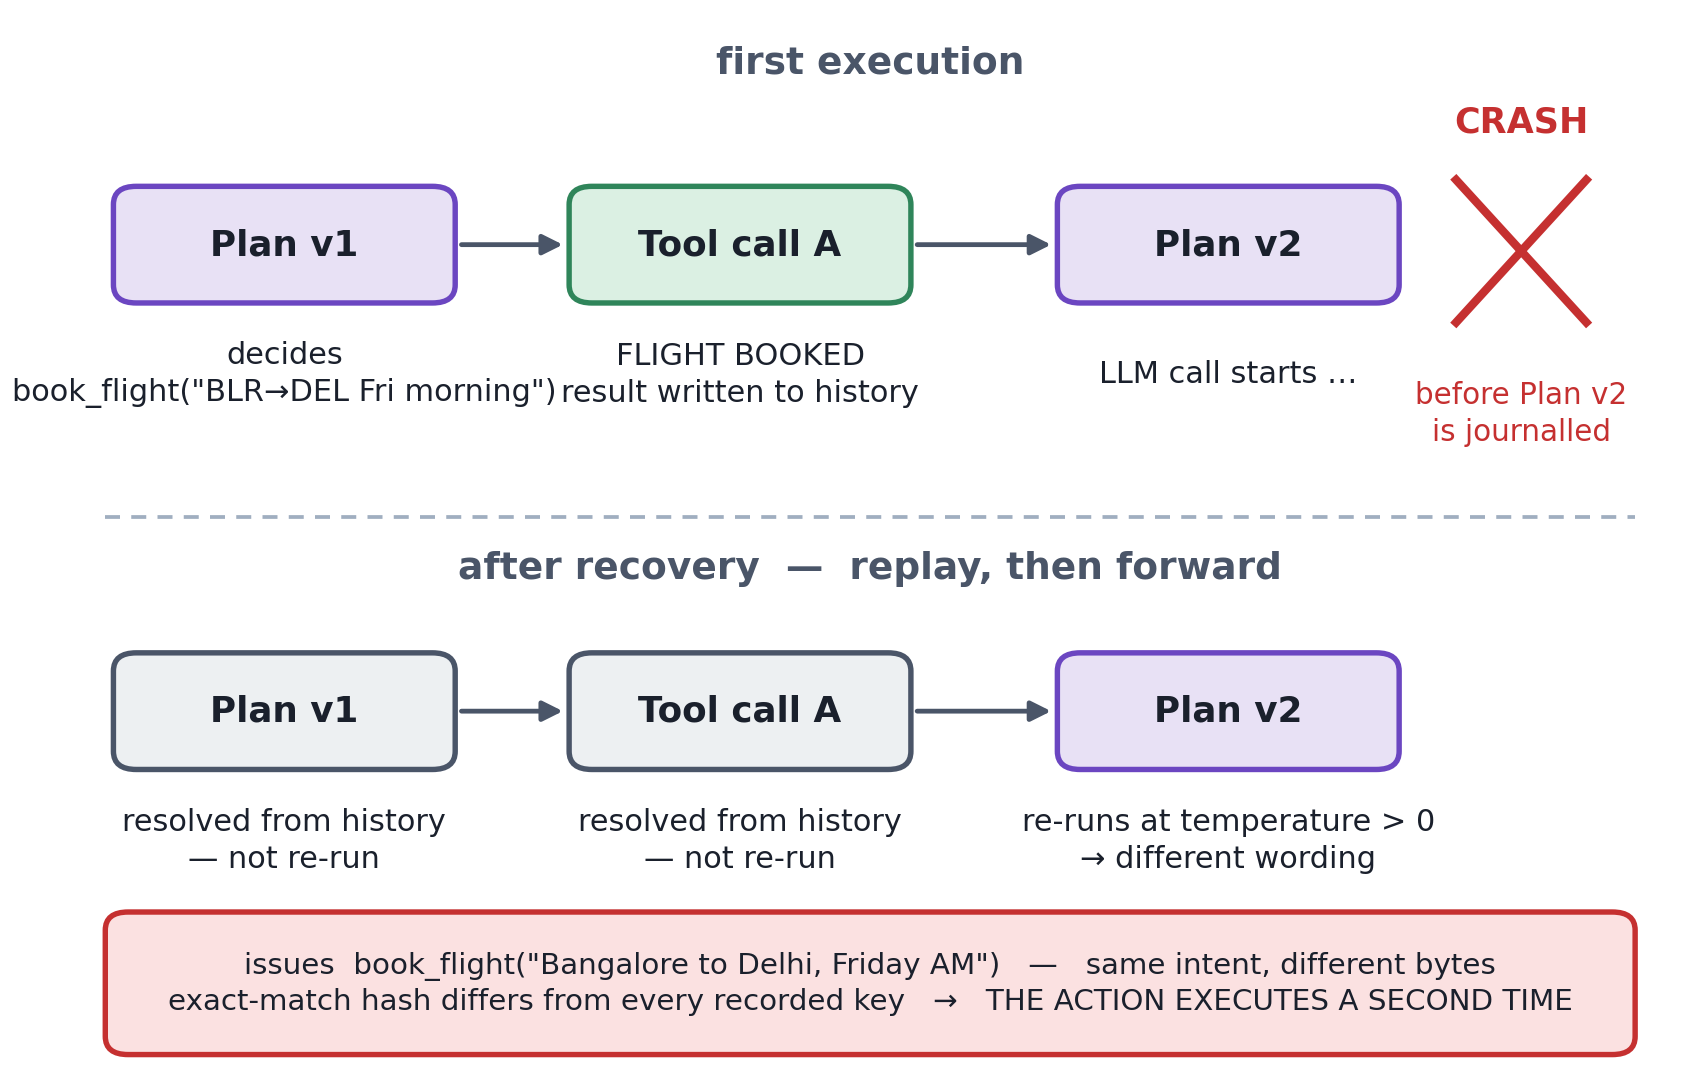
\includegraphics[width=\linewidth]{figures/fig_2_2_semantic_gap.png}
  \caption{The crash-induced, semantically duplicate side effect that
    exact-match idempotency cannot detect. Completed steps resolve from
    history and are not re-run, but a planning step that re-executes at a
    non-zero sampling temperature re-issues the same intent in different
    words, producing a hash that matches no recorded key.}
  \label{fig:semanticgap}
\end{figure}

\section{Identified Research Gap}

The gap this project addresses can be stated in a single sentence.

\begin{quote}
Every work in the semantic-caching literature applies embedding similarity to
decide whether to skip \emph{recomputing an answer}; none applies it to decide
whether to skip \emph{re-executing a side-effecting action} inside a durable
execution engine.
\end{quote}

The distinction is not cosmetic, because the consequence structure of a wrong
decision is entirely different. A semantic cache that returns a wrong hit
costs the user an inaccurate answer and costs the system nothing; the error is
recoverable and usually visible. A duplicate-suppression mechanism that
returns a wrong hit silently prevents a real-world action from occurring ---
a flight the user wanted is never booked, and nothing reports an error. Three
consequences follow, and they shape the design in Section~4.2.10:

\begin{enumerate}[leftmargin=*, itemsep=2pt]
  \item The threshold must be calibrated for a different and far more
    conservative error cost than a cache's, which is why the two-threshold
    design of~\cite{calibration2026} is adopted and why the mechanism is
    opt-in per activity rather than global.
  \item The verdict must be \emph{deterministic under replay}. A cache may
    recompute its decision freely; a durable execution engine may not, because
    a verdict that differed between the original execution and a replay would
    break the invariant on which the entire engine rests. This requirement has
    no counterpart in the caching literature and is the technically
    interesting part of the design.
  \item The verdict must be \emph{auditable after the fact}. When a mechanism
    is empowered to suppress real-world actions, the ability to answer ``why
    did this not happen?'' with a stored row rather than a guess is not a
    convenience; it is what makes the feature deployable at all.
\end{enumerate}

Table~\ref{tab:positioning} summarises how this work is positioned against the
closest prior art in each area.

\begin{table}[htbp]
  \centering
  \caption{Positioning of this work against the closest prior art}
  \label{tab:positioning}
  \small
  \begin{tabular}{@{}p{0.9in}p{1.48in}p{1.4in}p{1.24in}@{}}
    \toprule
    \textbf{Area} & \textbf{Closest prior art} & \textbf{What it does} &
    \textbf{What this work does} \\
    \midrule
    Durable execution & DBOS~\cite{dbos2025} &
      Postgres-backed, single node & Same substrate, partitioned across nodes \\
    Partitioning & Shard Manager~\cite{shardmanager2021} &
      Two-level mapping with ZooKeeper & Two-level mapping, no coordinator \\
    Ownership & Fencing tokens~\cite{kleppmann2017} &
      Resource rejects stale tokens & Check moved inside the write transaction \\
    Compensation & RAC~\cite{rac2026} &
      Undoes agent actions after failure & Prevents the duplicate before it runs \\
    Deduplication & GPTCache~\cite{gptcache2023} &
      Skips recomputing an answer & Skips re-executing a side effect \\
    Calibration & vCache~\cite{vcache2026} &
      Shows one cut-off is insufficient & Reproduced independently and reported \\
    \bottomrule
  \end{tabular}
\end{table}
